\subsection{Background information}
\label{sec:gbb-unfoldingintro}

We unfold data to the space jet level phase space as defined in reco-level, i.e. same requirements of jet kinematics and multiplicity. To unfold the data, we need to correct the detector response for the reconstructed distribution, which is measured by our detector. As such distribution is usually summarized by histograms, without loss of generality, we denote it as $y_i$. We also assume at this stage the reconstructed distribution has the background subtracted. For the true distribution we are interested in, let us denote it as $x_i$, its transformation into the reconstructed distribution should be represented as: $T_{ij}e_ix_i = y_j (1-f_j)$, where $e_i$ is the efficiency factor, $f_j$ is the fake rate and $T_ij$ is the response matrix. The efficiency factor accounts for the efficiency loss of a true particle ending up outside the reco-level fiducial region. The fake factor corrects for the effect of reconstructed events originating from outside the targeted truth level fiducial region. The response matrix can be thought as a bin transition matrix between reco and truth-level quantities both of which within their proper fiducial region.

The estimation of efficiency factor and fake rates is relatively simple as they are vectors which we directly take them from MC. The estimation of $U_{ij}=T_{ij}^{-1}$, i.e. the unfolding matrix, is difficult as it involves matrix inversion which is subject to instability and large uncertainties arising from potential degeneracy. Instead, we take a Bayesian approach invented by ~\cite{D'Agostini:1994zf}, to directly estimate the unfolding matrix itself. In the language of probability and by Bayes rule, we know that

\begin{equation}
  U_{ij} = \mathrm{P}(x_i|y_j) = \frac{\mathrm{P}(y_j|x_i)\mathrm{P}(x_i)}{\sum_i \mathrm{P}(y_j|x_i)\cdot \mathrm{P}(x_i)}
  \label{eqn:unfolding:final}
\end{equation}

where $x_i$ and $y_j$ are efficiency and fake corrected true and reconstructed distributions, and $\mathrm{P}(y_j|x_i)$ are the response matrix entries. The data truth priors $\mathrm{P}(x_i)$, are not known to us but can be approximated by the MC truth distributions to start with. Through iterative procedure and using the output unfolded distribution as the next step prior, one can lower the bias once the result has converged. For this analysis the package that executes the Bayesian iterative unfolding is \texttt{RooUnfold} 1.1.1~\cite{Adye:2011gm}.

The following sections describe the details of unfolding with respect to the $g\rightarrow b\bar{b}$  measurement. Sec.~\ref{sec:gbb-unfolding:inputquantities} contains the input quantities used for unfolding: the unfolding matrices and the fake and inefficiency factors. The systematic uncertainties related to the unfolding procedure are described in Sec.~\ref{sec:gbb-systs:unfolding}. Technical closure and unfolding iteration optimization are documented in Sec.~\ref{app:gbb-unfolding:technicalclosure} and Sec.~\ref{app:gbb-unfolding:optimization} respectively.  


\subsection{Response matrices and acceptance factors}
\label{sec:gbb-unfolding:inputquantities}

The fake and efficiency factors are shown in Fig.~\ref{fig:gbb-acceptance} and Fig.~\ref{fig:gbb-fake}, respectively.  As expected, the factors are largely independent of the variables; there is a small decrease at low values in Fig.~\ref{fig:gbb-fake} in cases where the second sub-jet is lost/merged.  The unfolding matrices are shown in Fig.~\ref{fig:gbb-responsematrix1}; as the track-jet angular and momentum resolutions are superb, the matrices are very diagonal especially for angular variables.

\begin{figure}[htpb!]
\begin{center}
  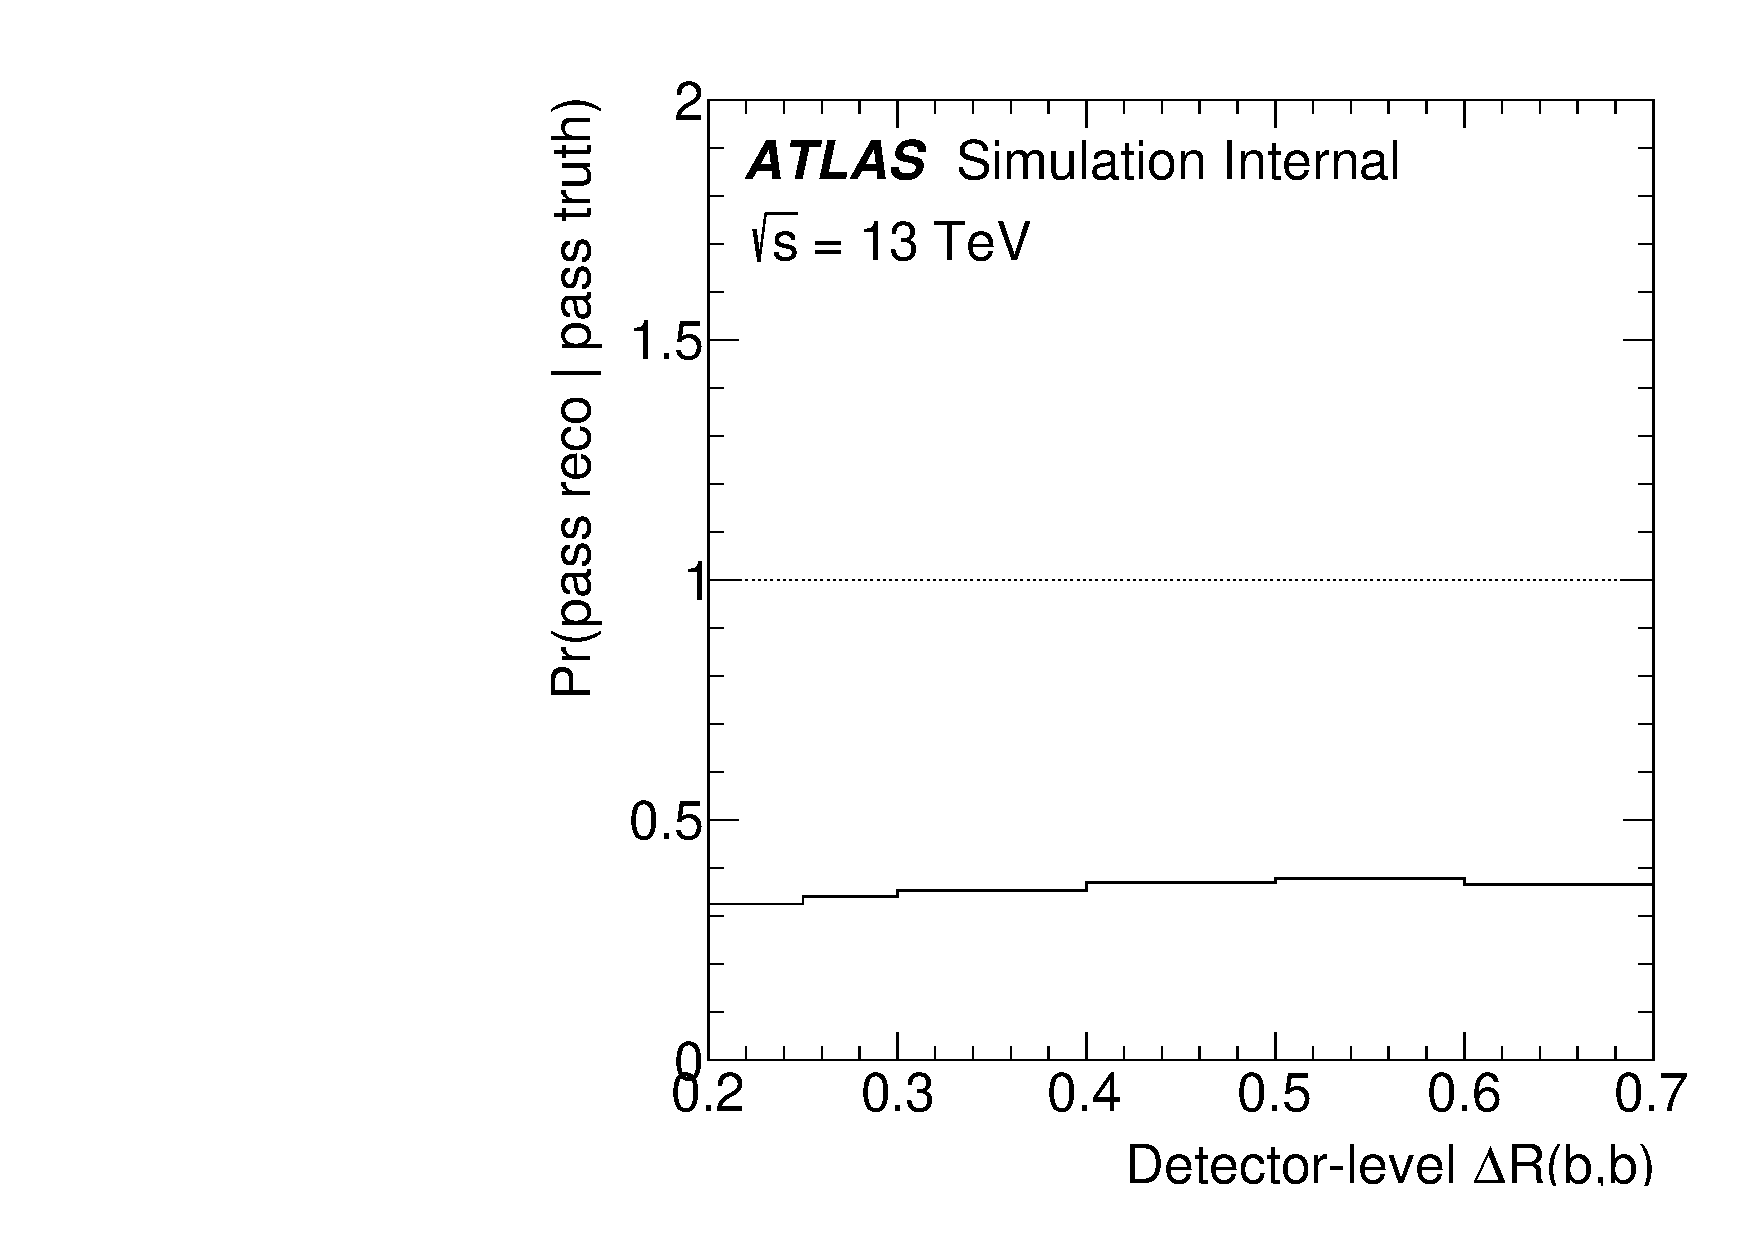
\includegraphics[width=0.23\linewidth]{figures/gbb/Unfolding/dR_effic_factor.pdf}
  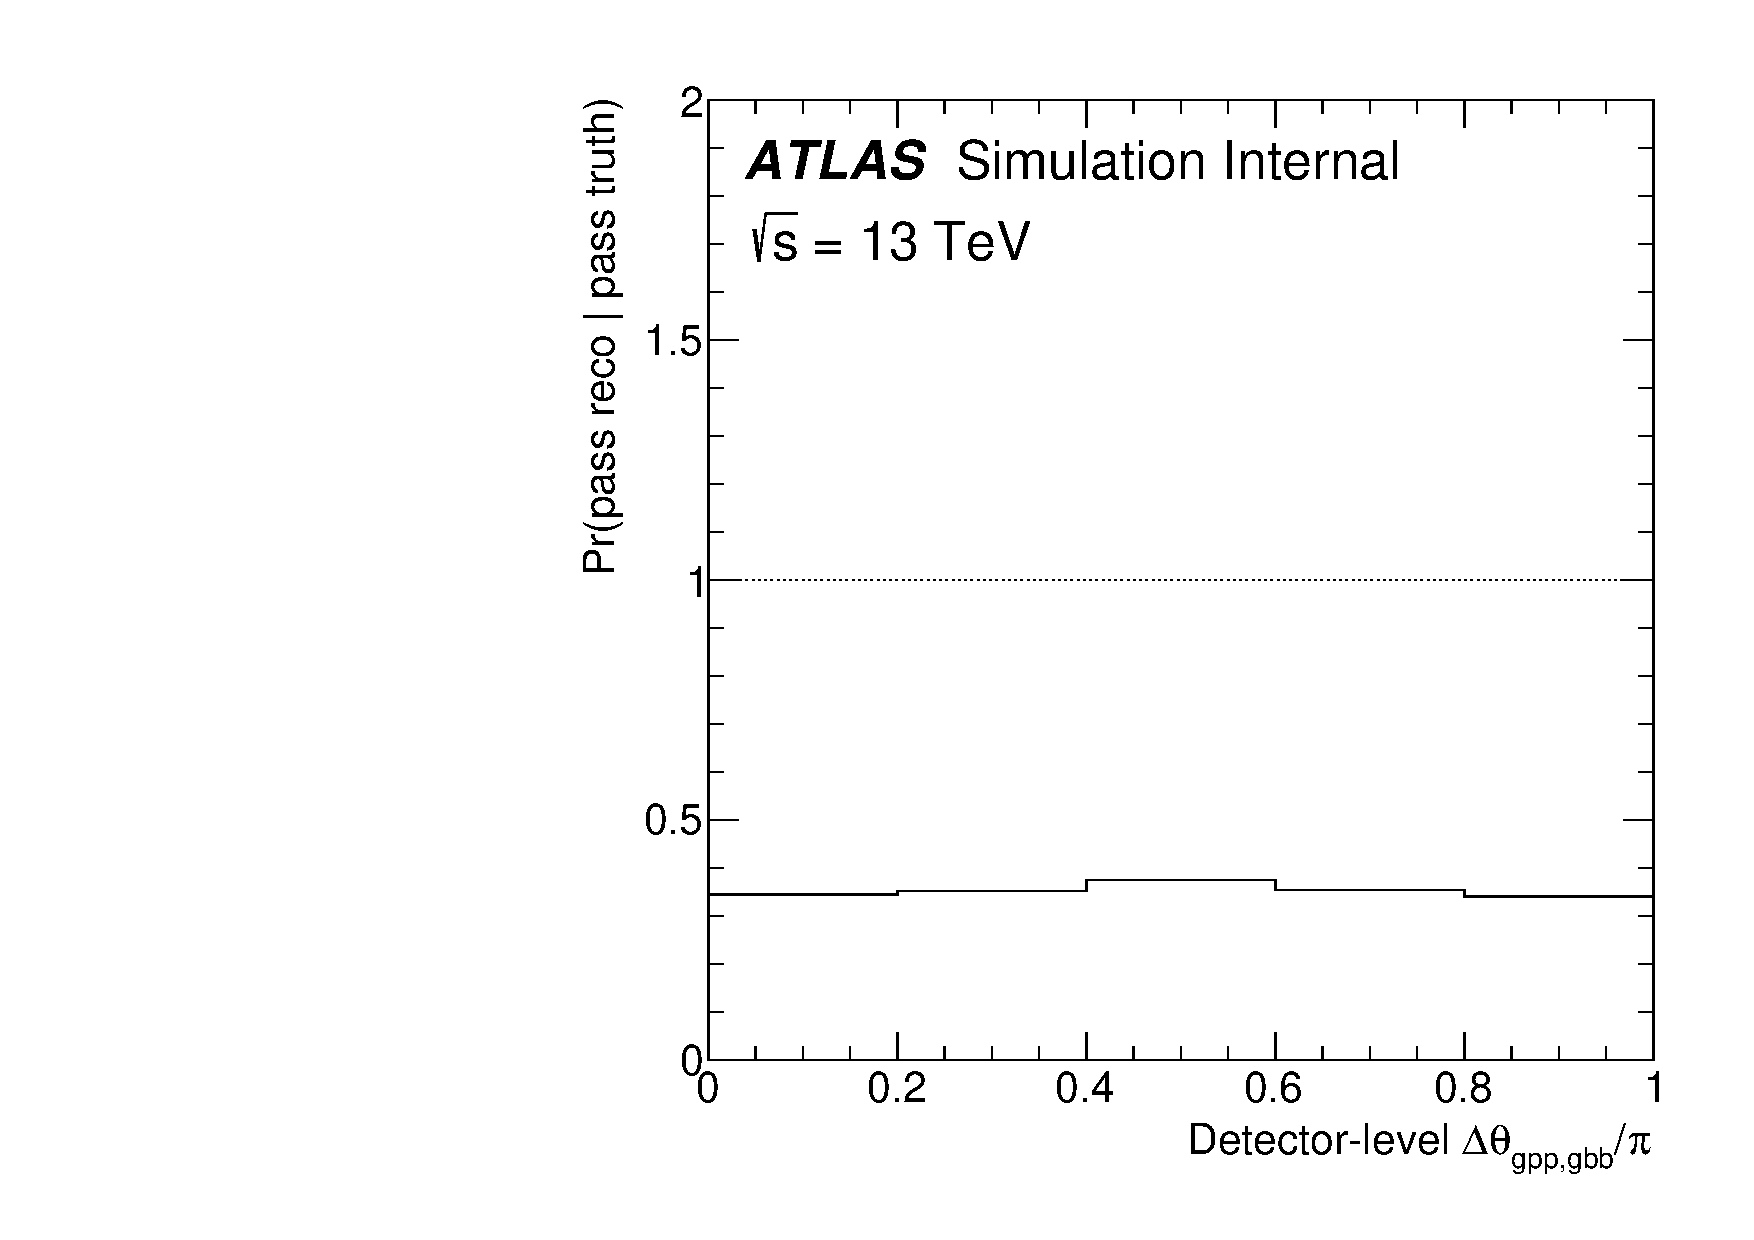
\includegraphics[width=0.23\linewidth]{figures/gbb/Unfolding/dphi_effic_factor.pdf}
  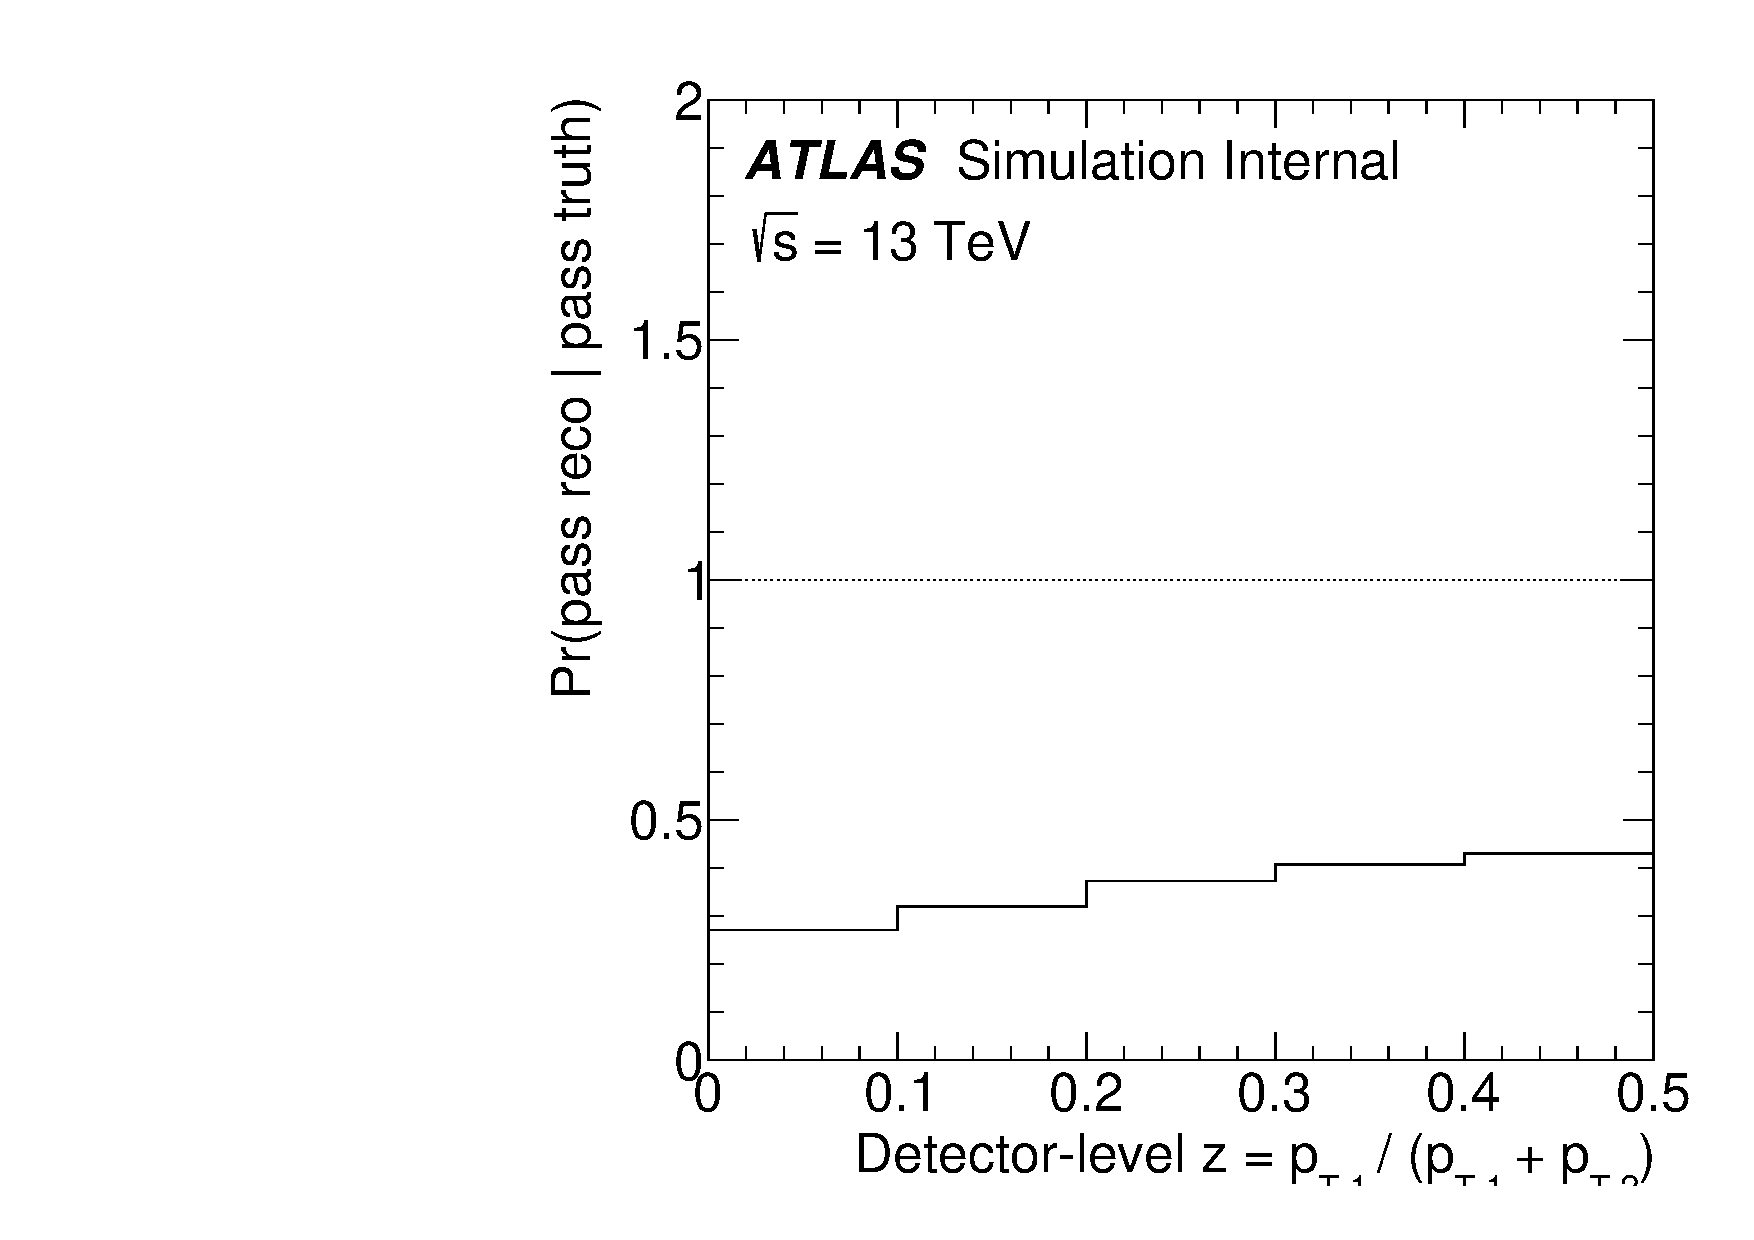
\includegraphics[width=0.23\linewidth]{figures/gbb/Unfolding/ZpT_effic_factor.pdf}
  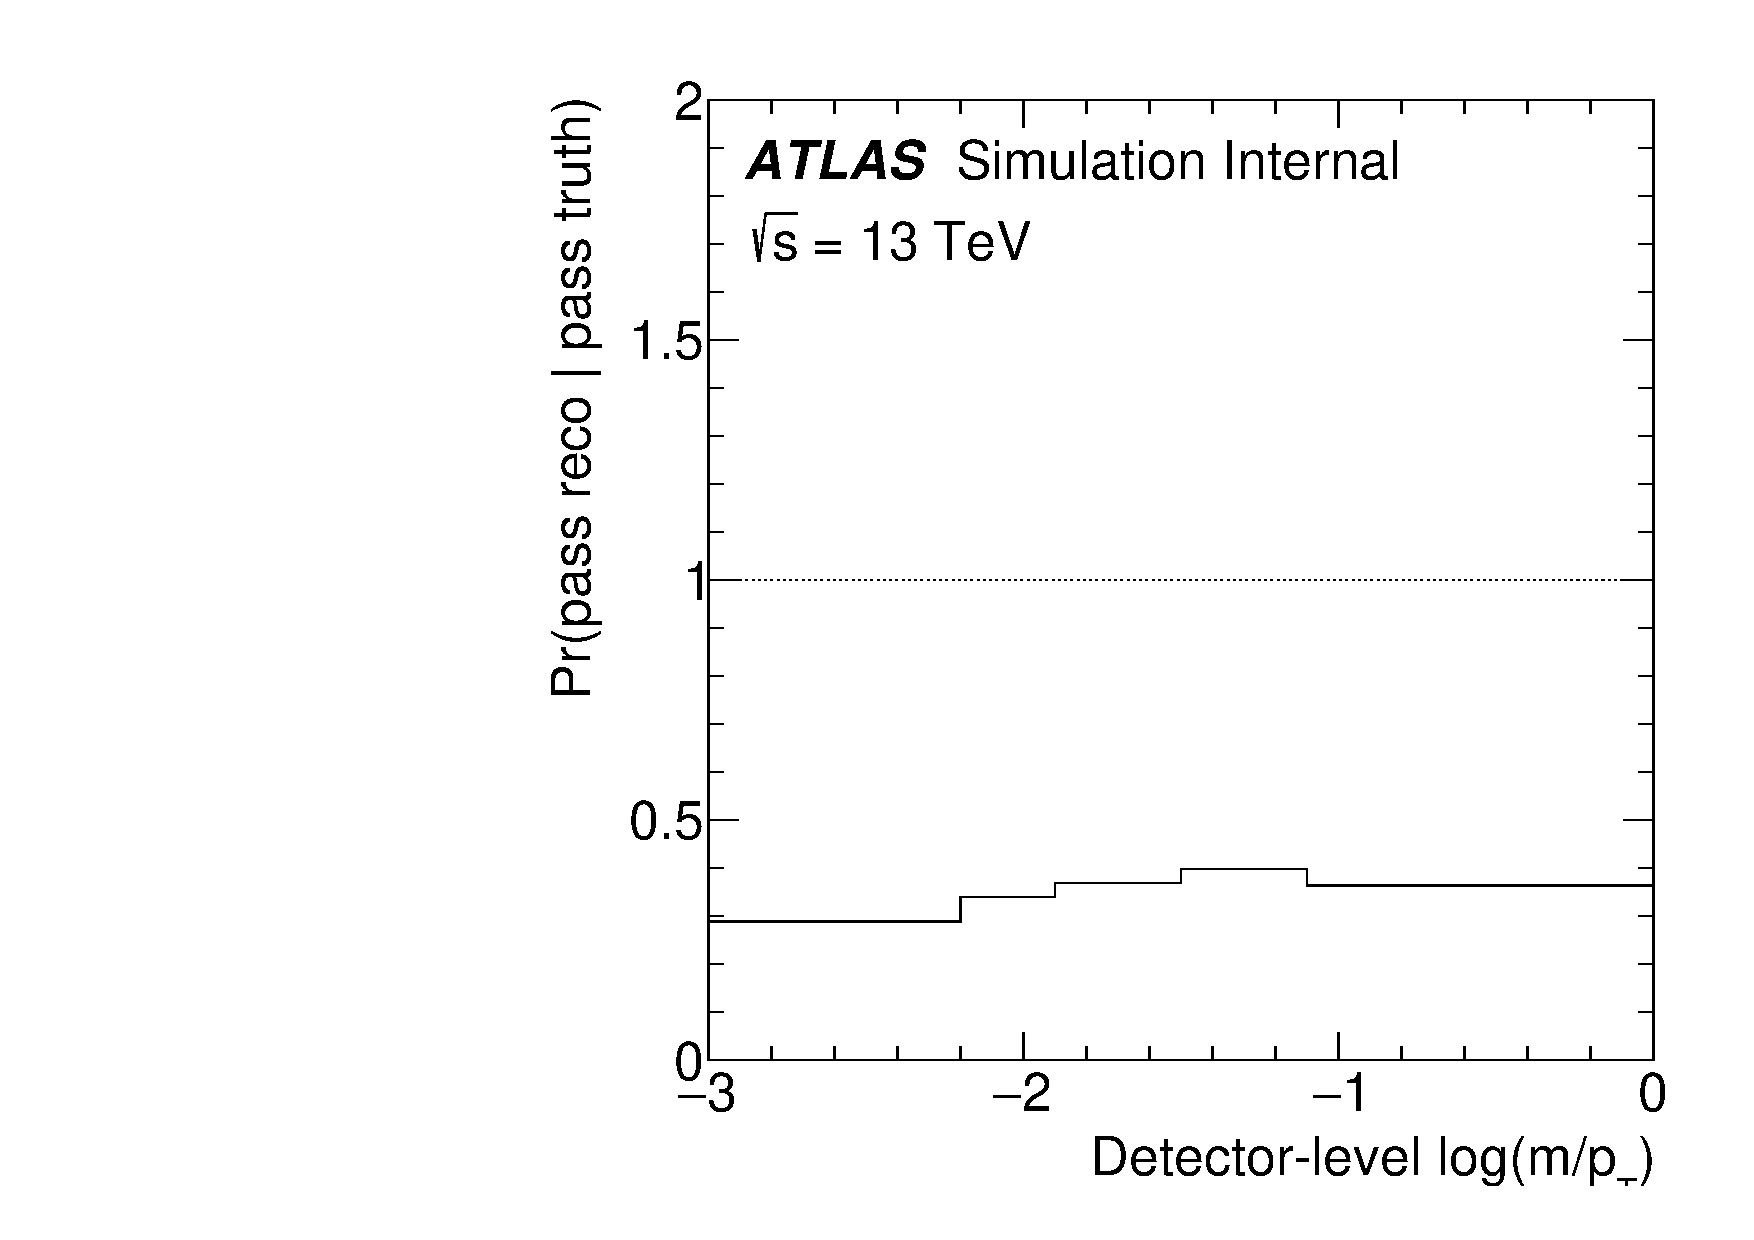
\includegraphics[width=0.23\linewidth]{figures/gbb/Unfolding/fracmasspt_effic_factor.pdf}
\caption[]{The efficiency factors as described in Sec.~\ref{sec:gbb-unfoldingintro}.} 
\label{fig:gbb-acceptance}
\end{center}
\end{figure}

\begin{figure}[htpb!]
\begin{center}
  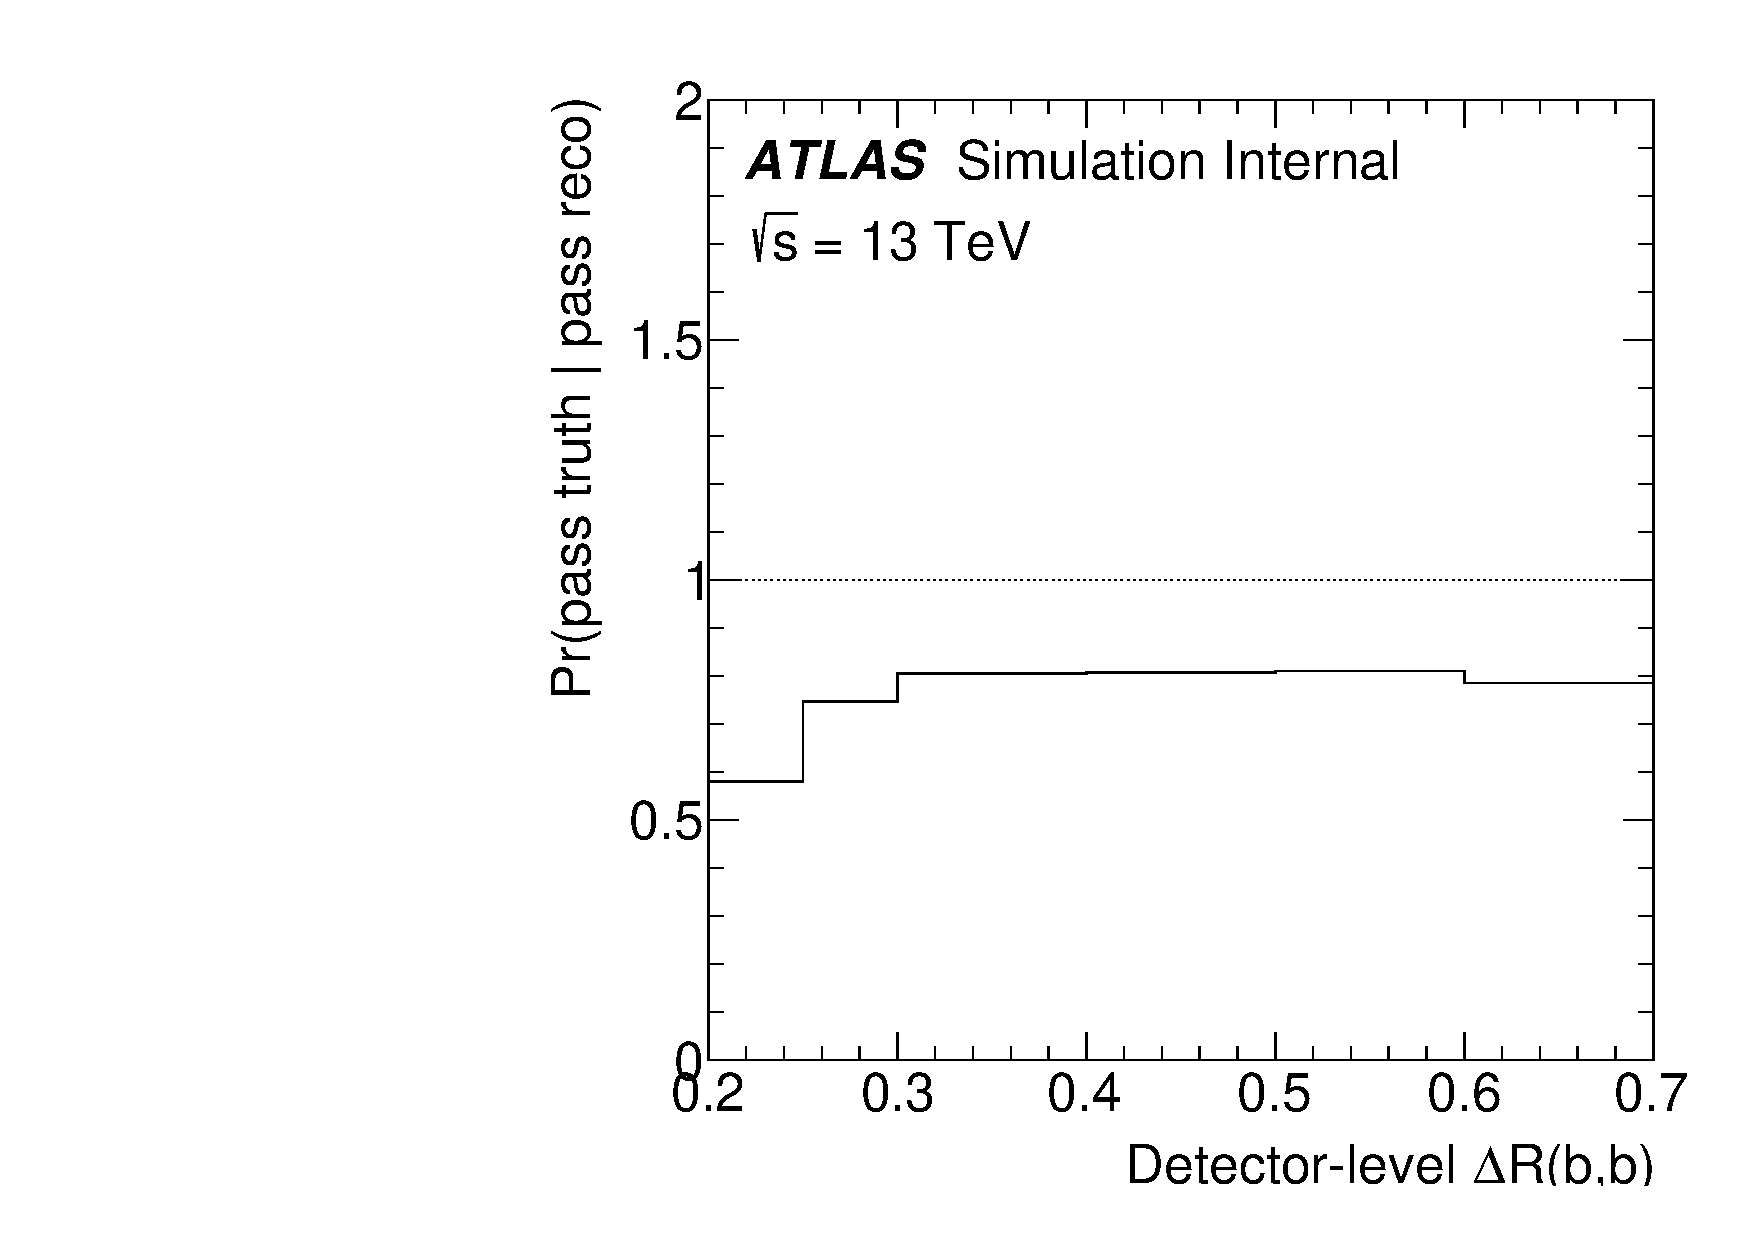
\includegraphics[width=0.23\linewidth]{figures/gbb/Unfolding/dR_fake_factor.pdf}
  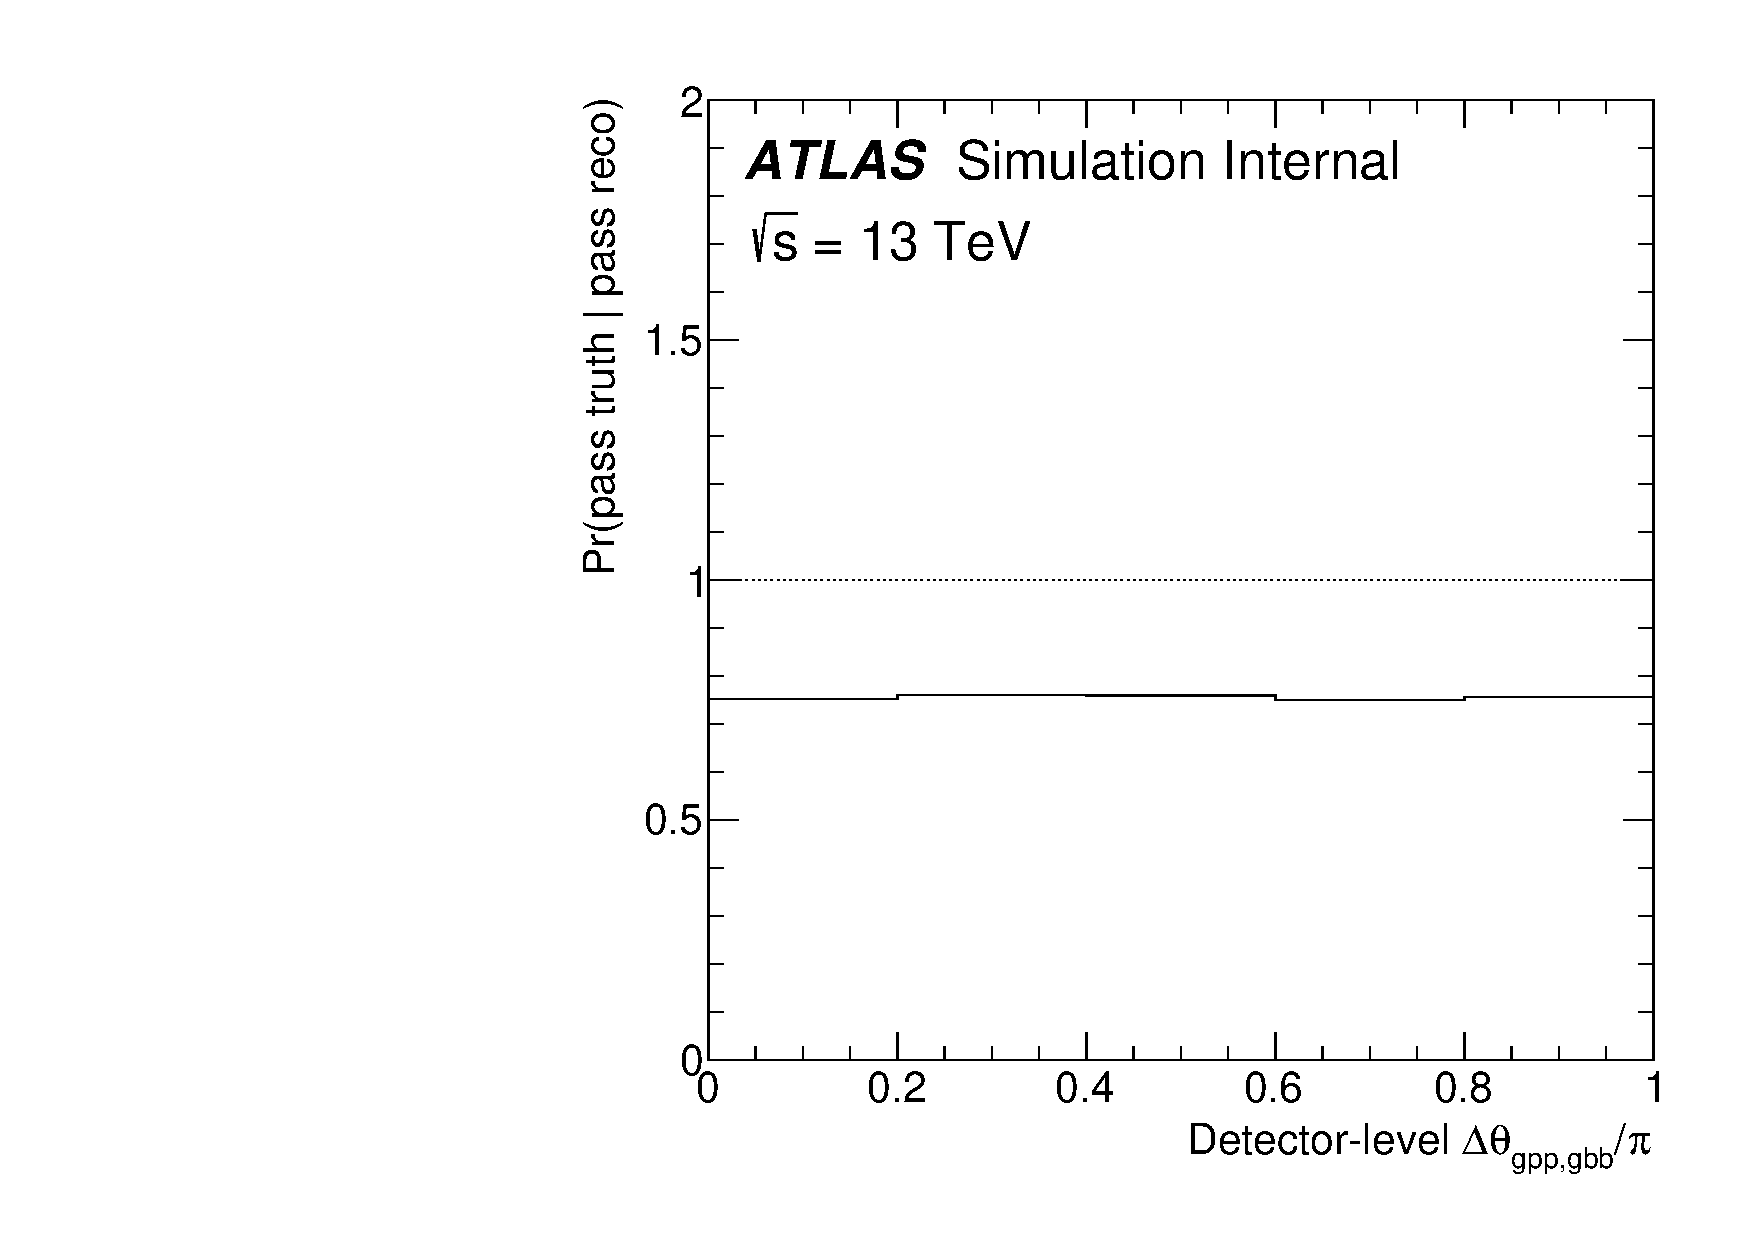
\includegraphics[width=0.23\linewidth]{figures/gbb/Unfolding/dphi_fake_factor.pdf}
  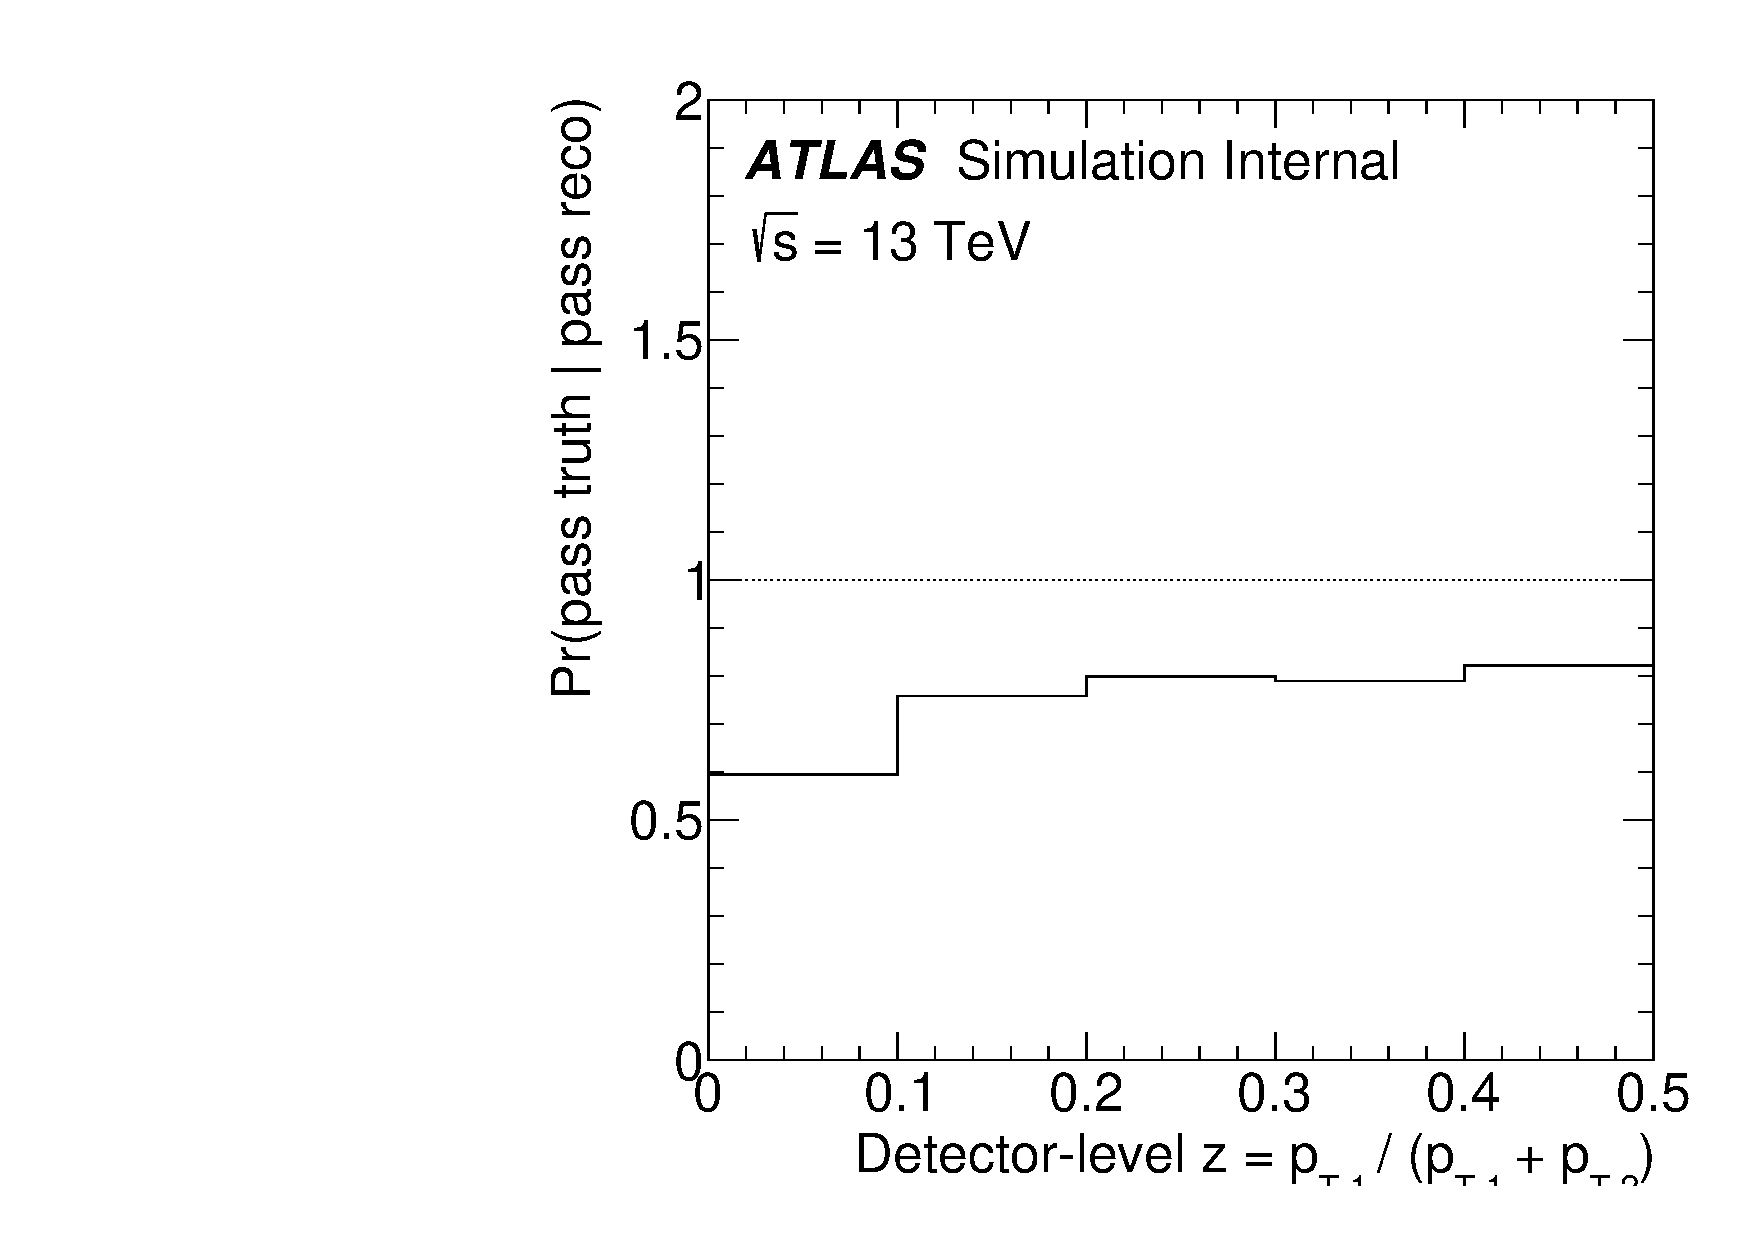
\includegraphics[width=0.23\linewidth]{figures/gbb/Unfolding/ZpT_fake_factor.pdf}
  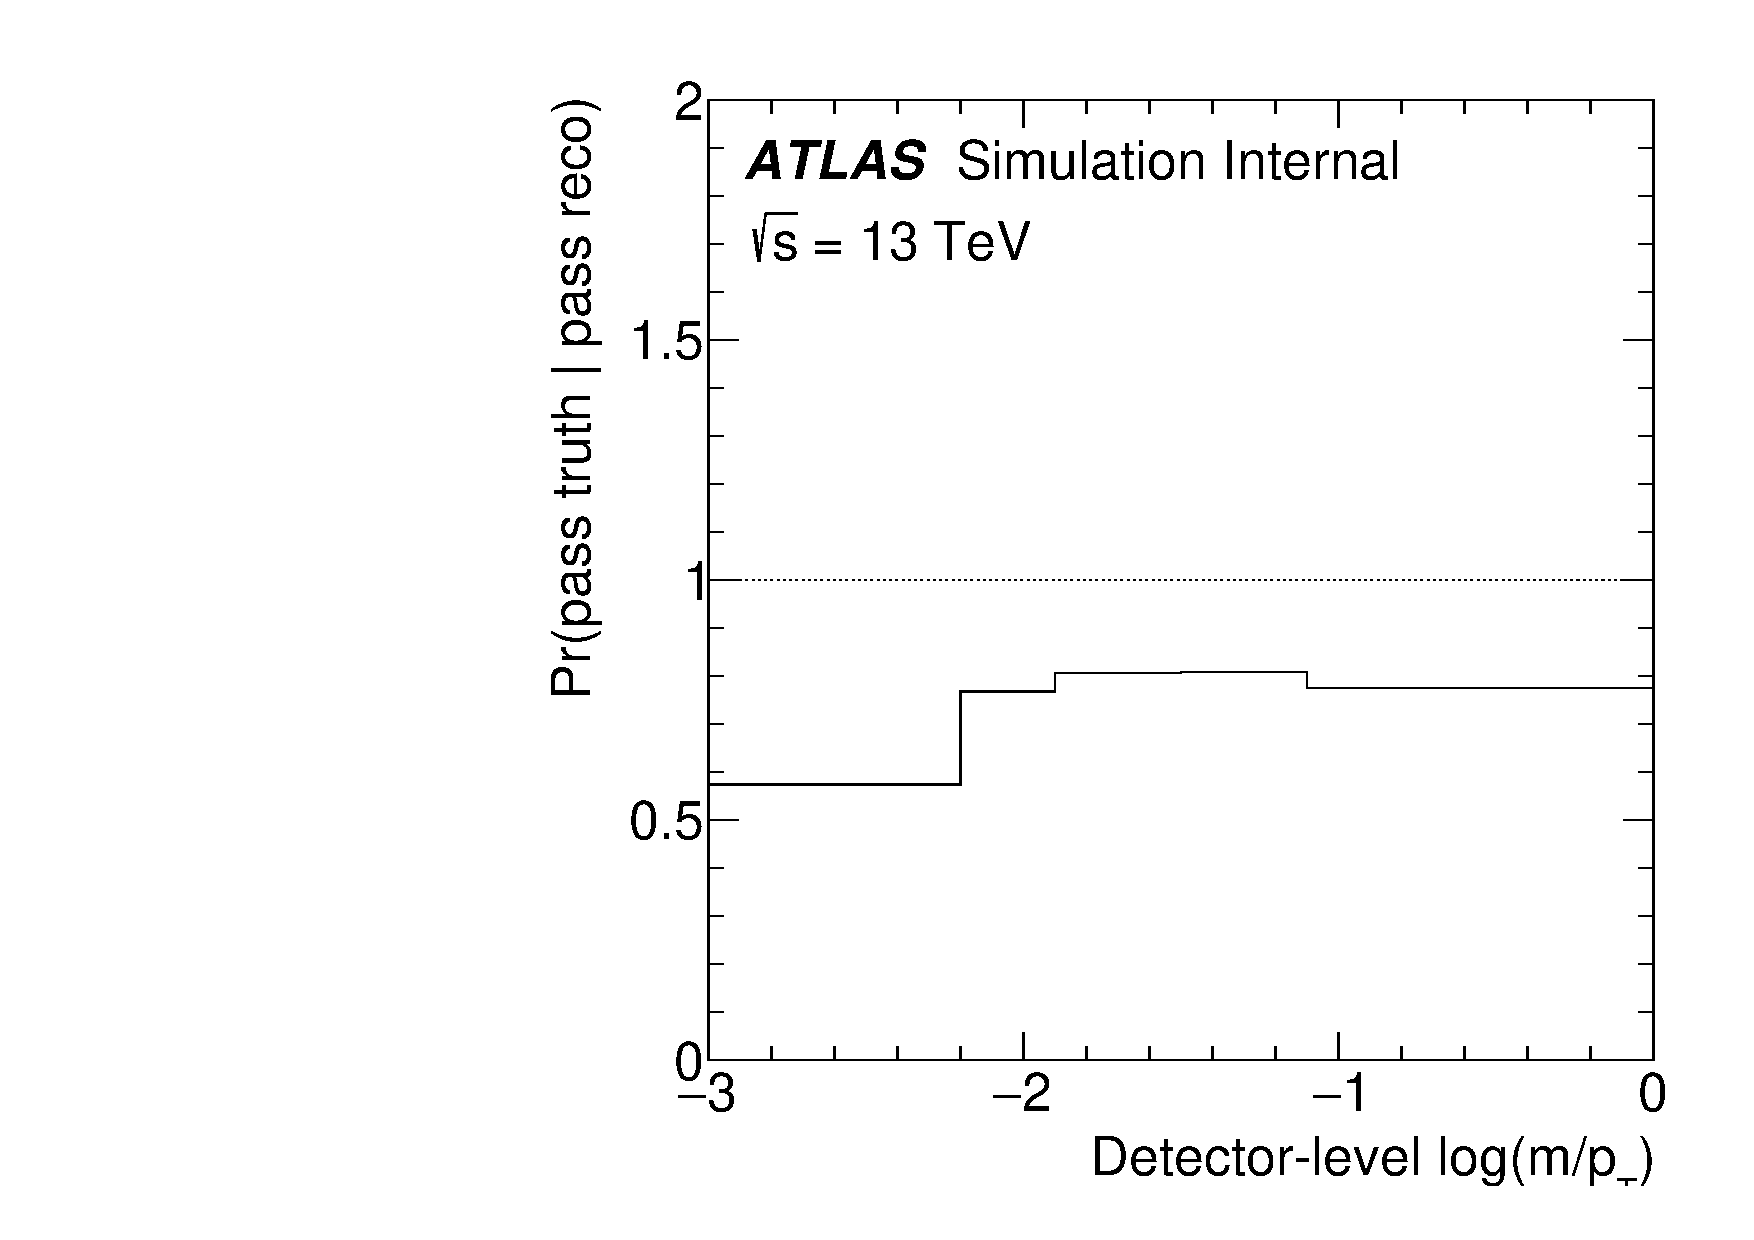
\includegraphics[width=0.23\linewidth]{figures/gbb/Unfolding/fracmasspt_fake_factor.pdf}
\caption[]{The fake factors as described in Sec.~\ref{sec:gbb-unfoldingintro}.} 
\label{fig:gbb-fake}
\end{center}
\end{figure}

\begin{figure}[htpb!]
\begin{center}
  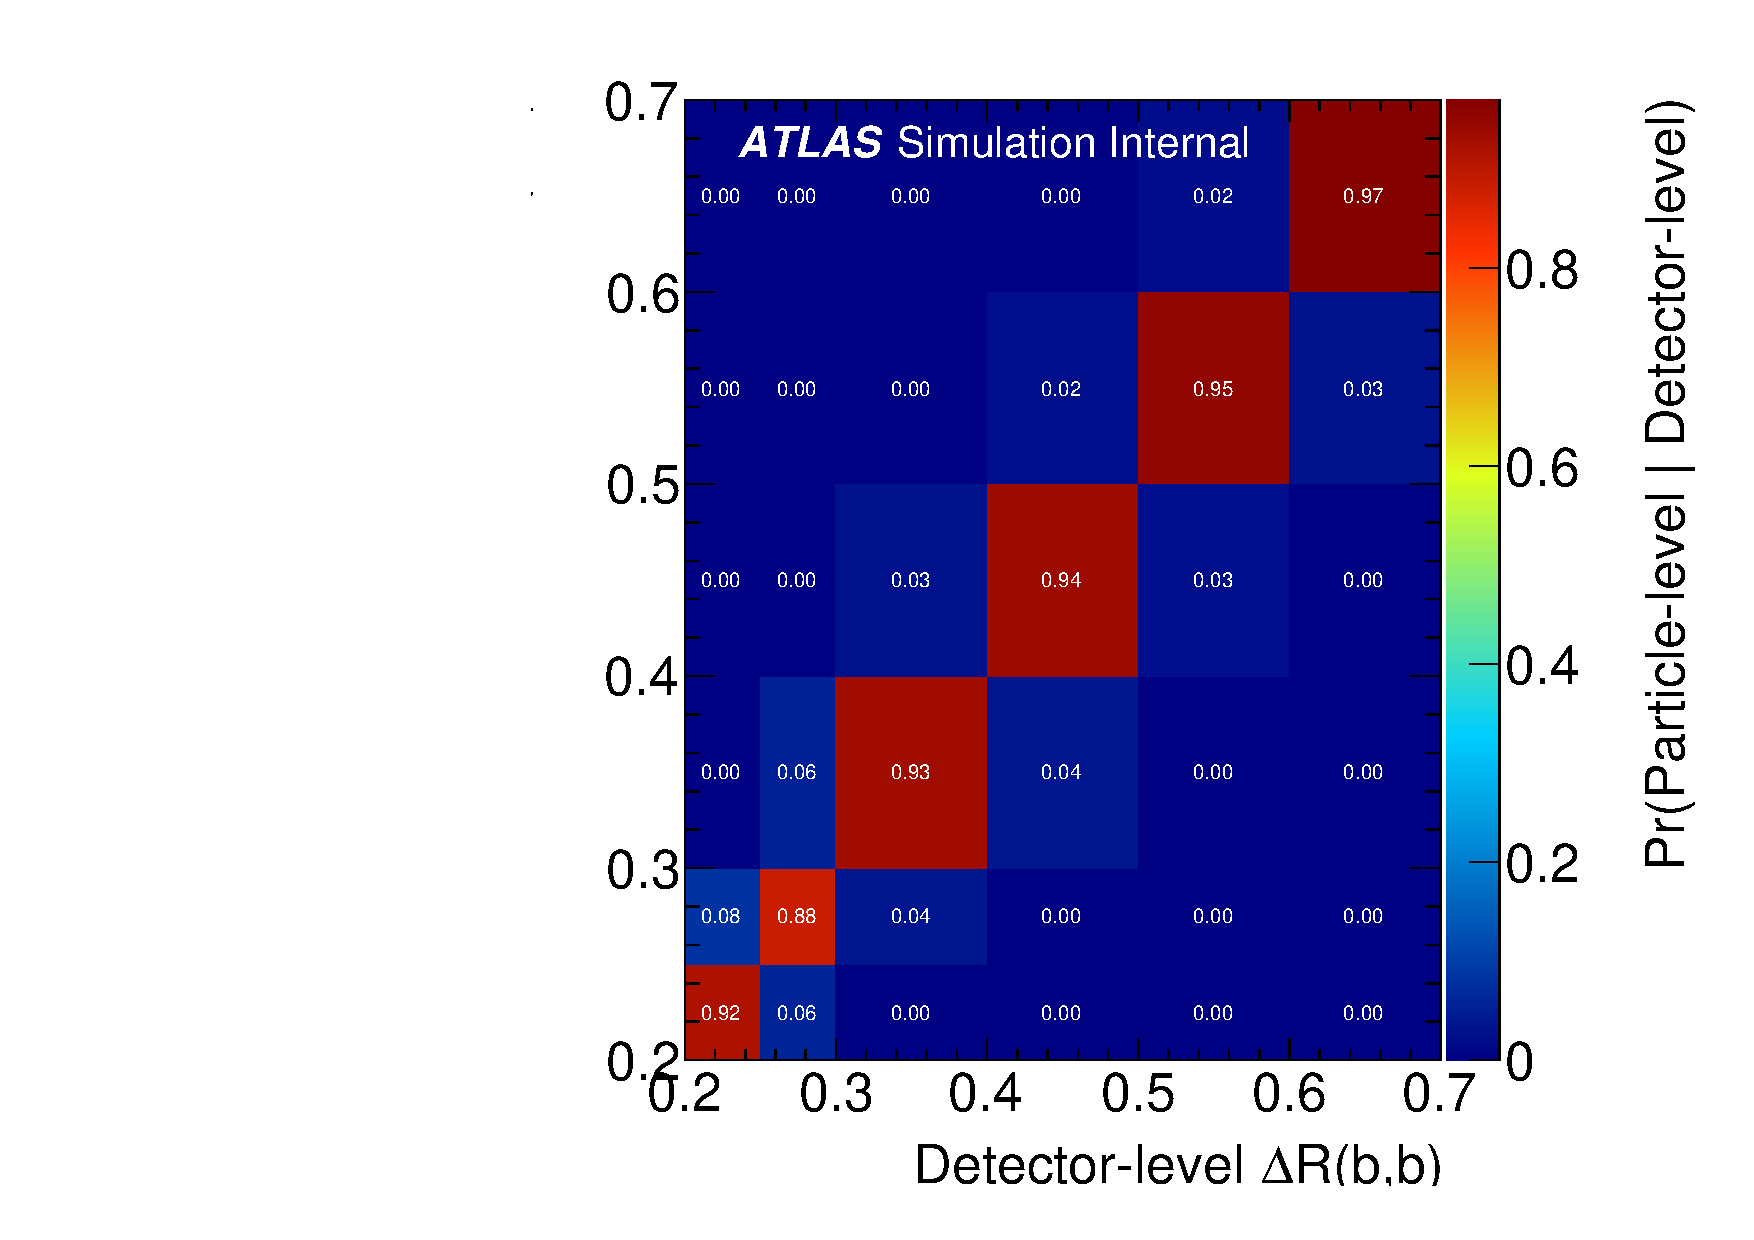
\includegraphics[width=0.4\linewidth]{figures/gbb/Unfolding/dR_ResponseMatrix_x.pdf}
  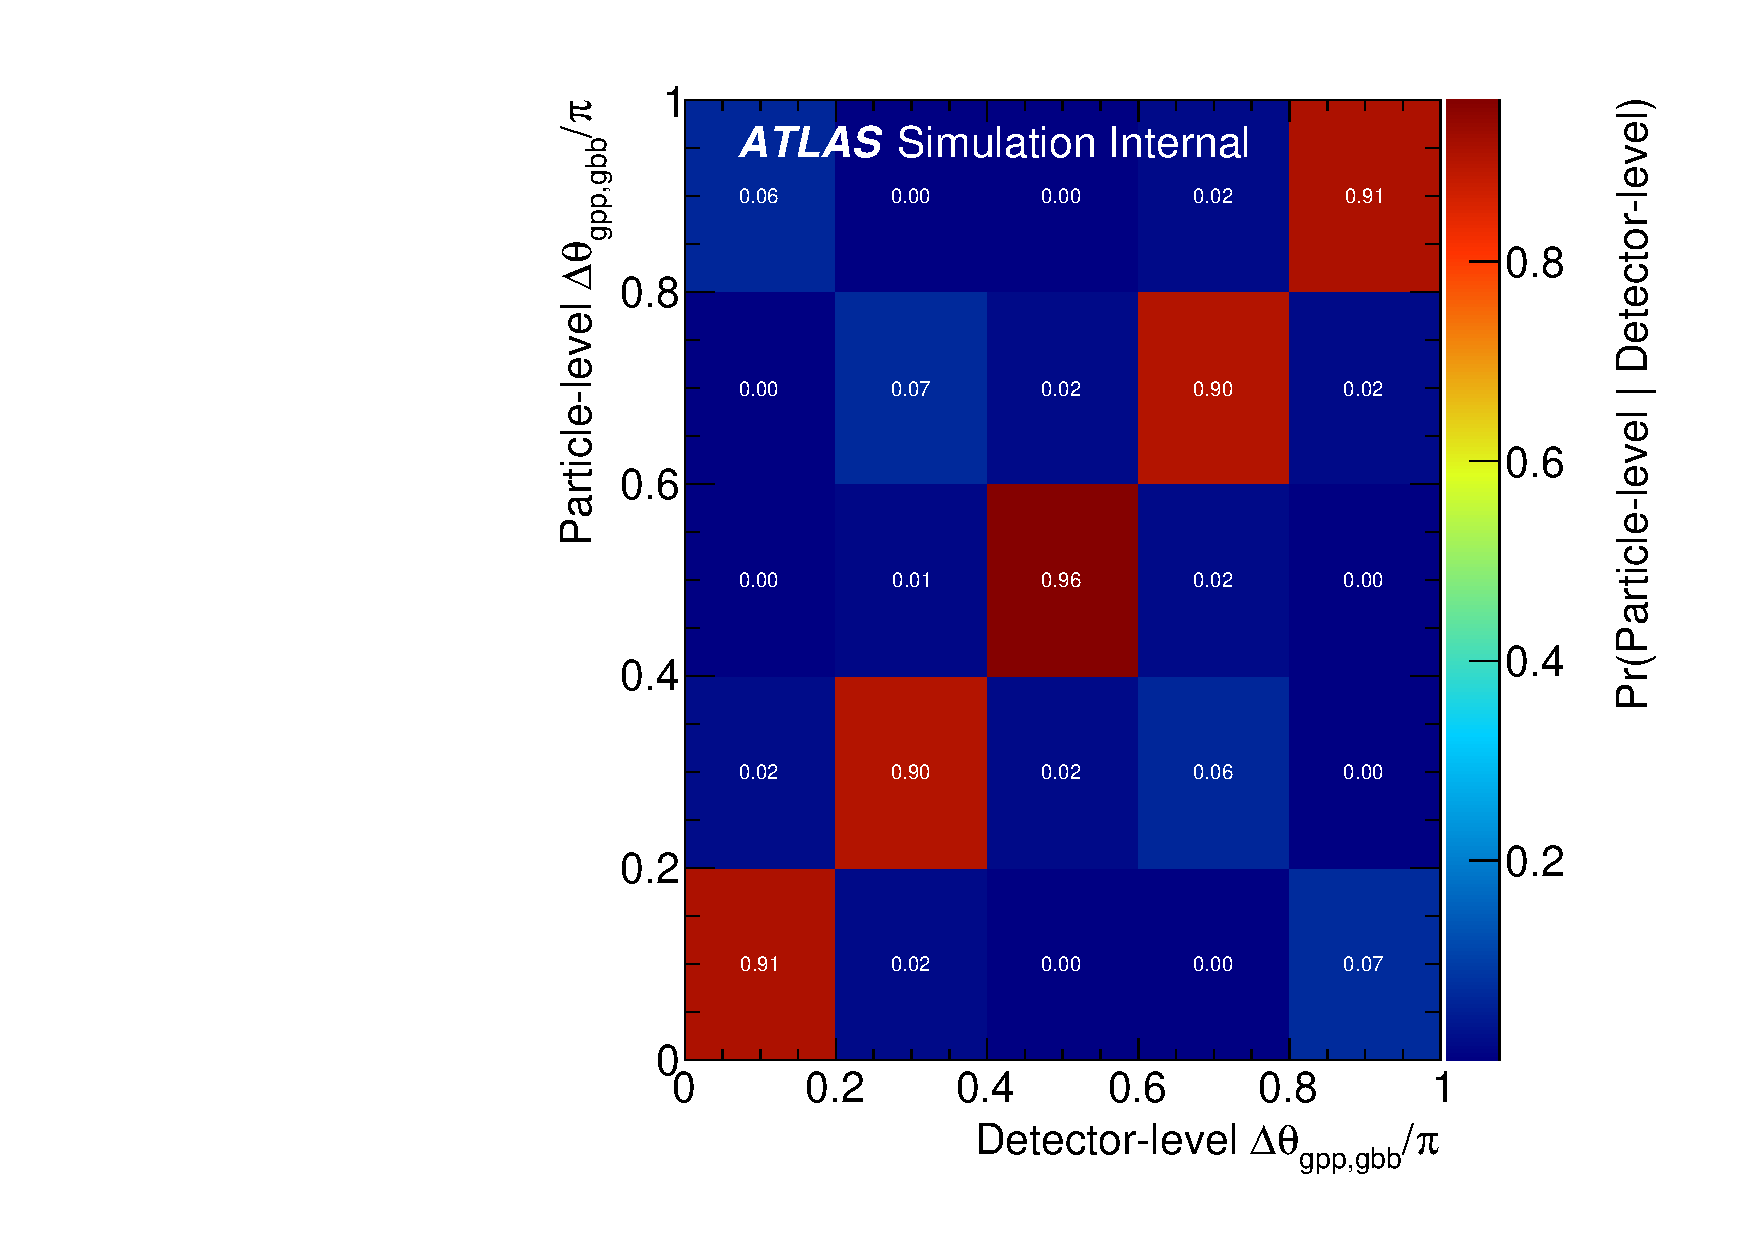
\includegraphics[width=0.4\linewidth]{figures/gbb/Unfolding/dphi_ResponseMatrix_x.pdf}
  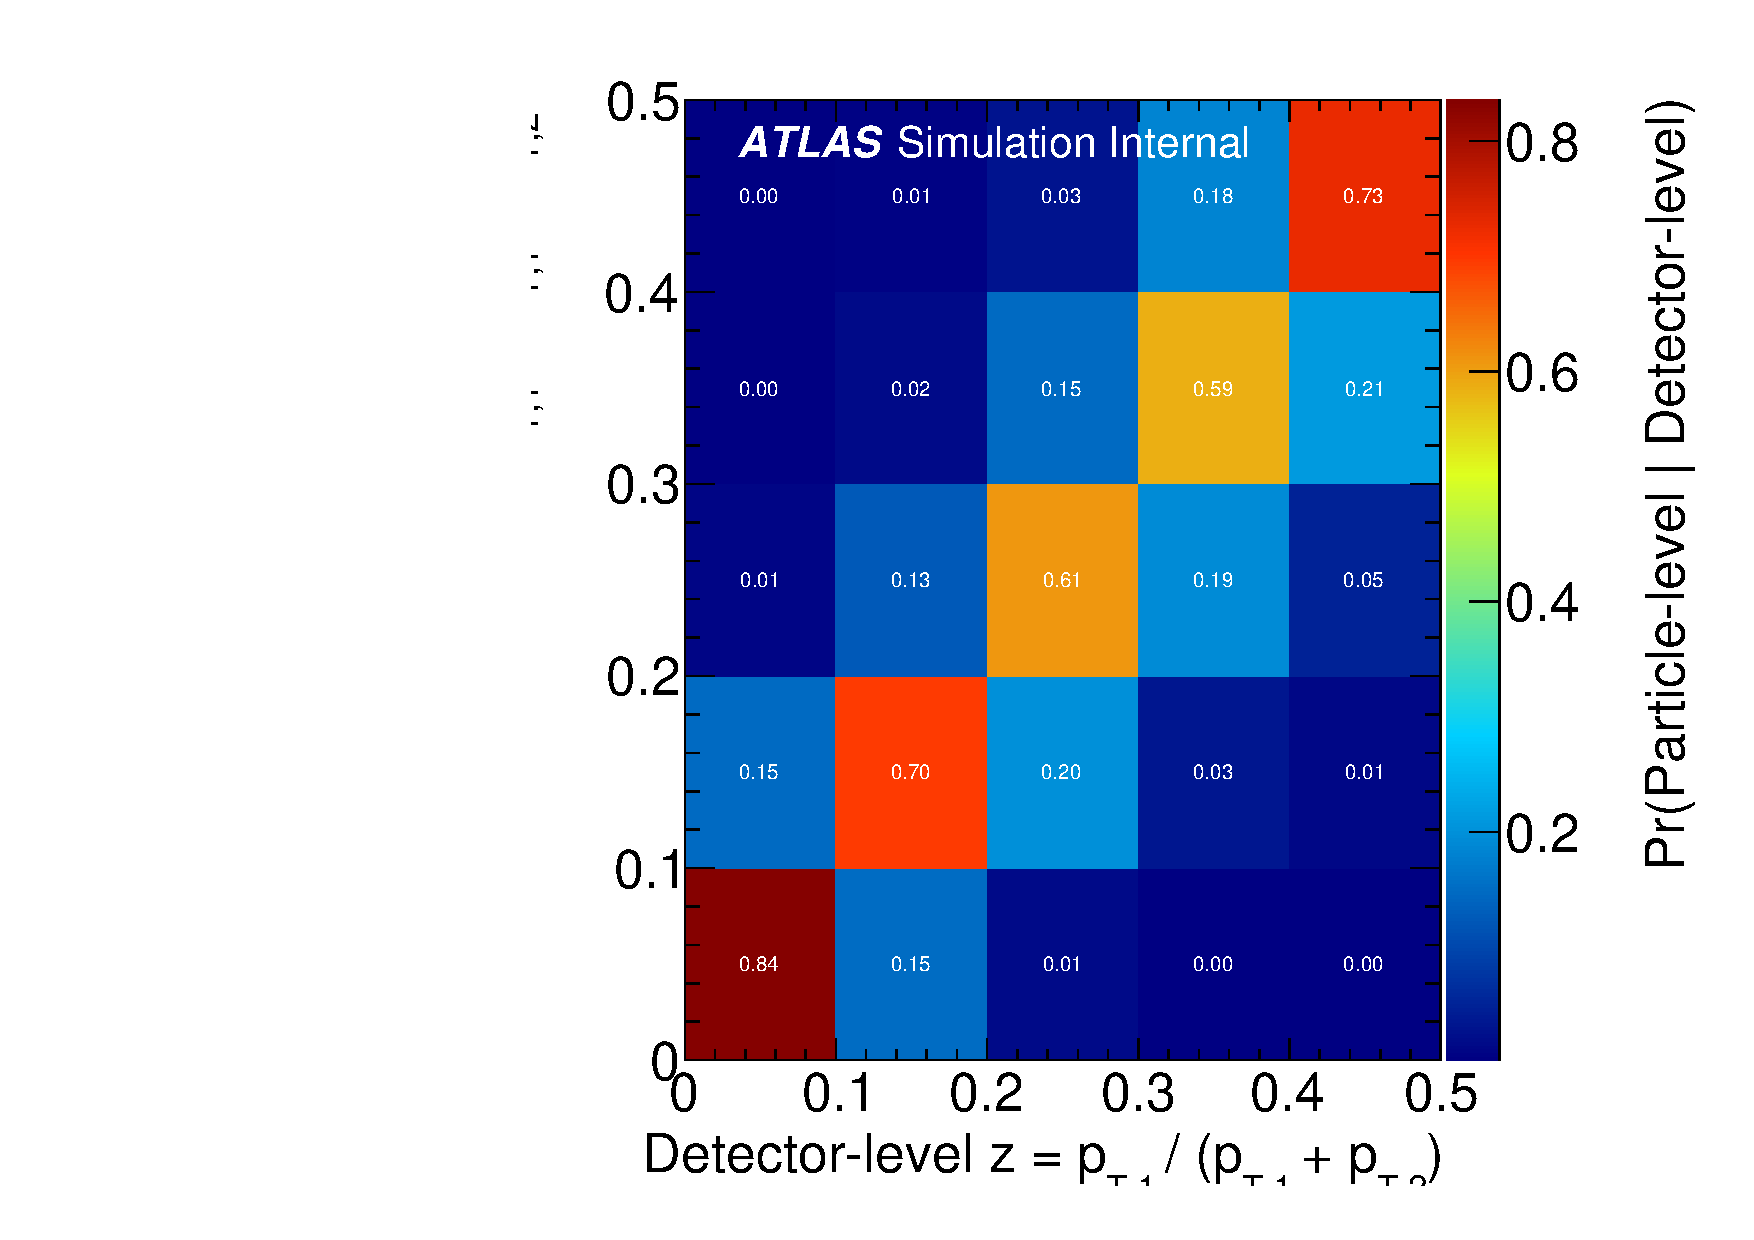
\includegraphics[width=0.4\linewidth]{figures/gbb/Unfolding/ZpT_ResponseMatrix_x.pdf}
  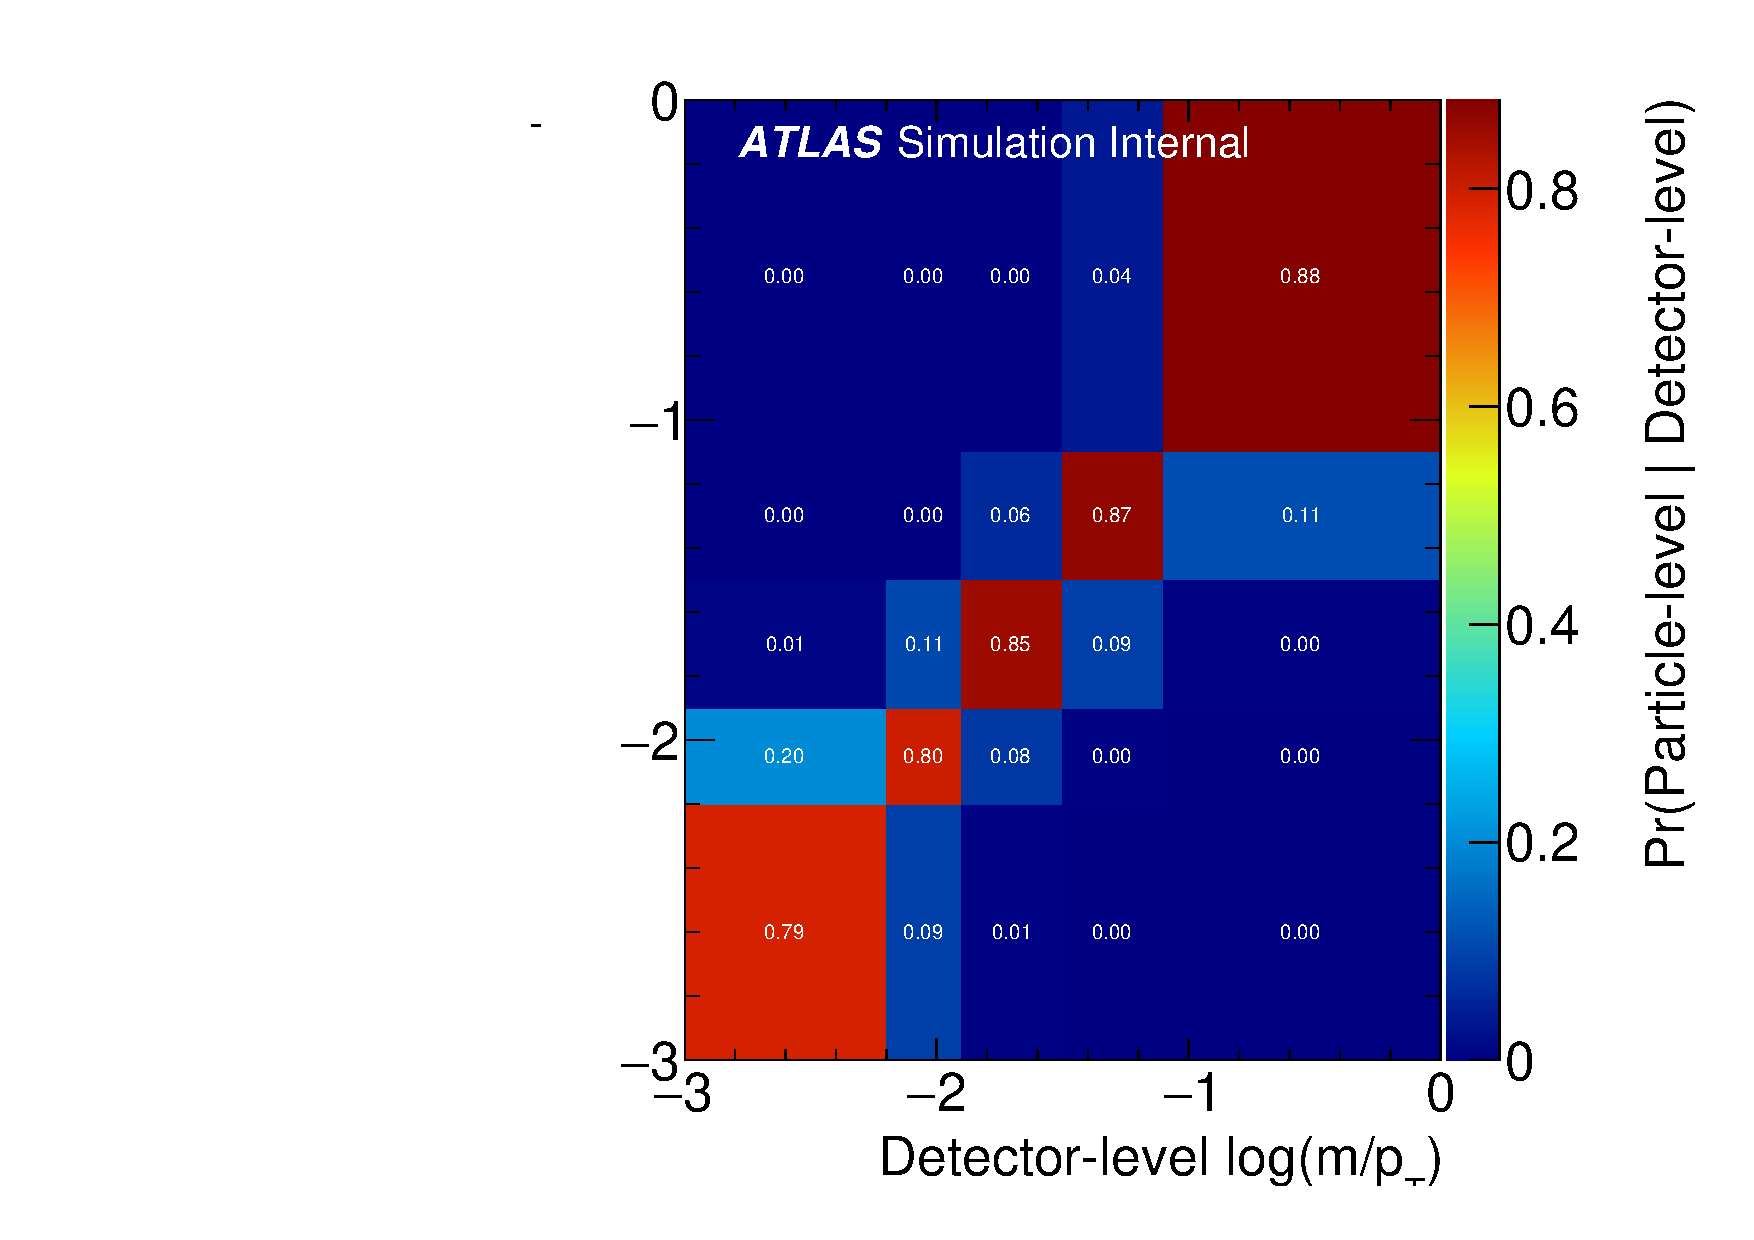
\includegraphics[width=0.4\linewidth]{figures/gbb/Unfolding/fracmasspt_ResponseMatrix_x.pdf}
\caption[]{The unfolding matrices.  } 
\label{fig:gbb-responsematrix1}
\end{center}
\end{figure}

\clearpage

